
%% bare_conf.tex
%% V1.3
%% 2007/01/11
%% by Michael Shell
%% See:
%% http://www.michaelshell.org/
%% for current contact information.
%%
%% This is a skeleton file demonstrating the use of IEEEtran.cls
%% (requires IEEEtran.cls version 1.7 or later) with an IEEE conference paper.
%%
%% Support sites:
%% http://www.michaelshell.org/tex/ieeetran/
%% http://www.ctan.org/tex-archive/macros/latex/contrib/IEEEtran/
%% and
%% http://www.ieee.org/

%%*************************************************************************
%% Legal Notice:
%% This code is offered as-is without any warranty either expressed or
%% implied; without even the implied warranty of MERCHANTABILITY or
%% FITNESS FOR A PARTICULAR PURPOSE! 
%% User assumes all risk.
%% In no event shall IEEE or any contributor to this code be liable for
%% any damages or losses, including, but not limited to, incidental,
%% consequential, or any other damages, resulting from the use or misuse
%% of any information contained here.
%%
%% All comments are the opinions of their respective authors and are not
%% necessarily endorsed by the IEEE.
%%
%% This work is distributed under the LaTeX Project Public License (LPPL)
%% ( http://www.latex-project.org/ ) version 1.3, and may be freely used,
%% distributed and modified. A copy of the LPPL, version 1.3, is included
%% in the base LaTeX documentation of all distributions of LaTeX released
%% 2003/12/01 or later.
%% Retain all contribution notices and credits.
%% ** Modified files should be clearly indicated as such, including  **
%% ** renaming them and changing author support contact information. **
%%
%% File list of work: IEEEtran.cls, IEEEtran_HOWTO.pdf, bare_adv.tex,
%%                    bare_conf.tex, bare_jrnl.tex, bare_jrnl_compsoc.tex
%%*************************************************************************

% *** Authors should verify (and, if needed, correct) their LaTeX system  ***
% *** with the testflow diagnostic prior to trusting their LaTeX platform ***
% *** with production work. IEEE's font choices can trigger bugs that do  ***
% *** not appear when using other class files.                            ***
% The testflow support page is at:
% http://www.michaelshell.org/tex/testflow/



% Note that the a4paper option is mainly intended so that authors in
% countries using A4 can easily print to A4 and see how their papers will
% look in print - the typesetting of the document will not typically be
% affected with changes in paper size (but the bottom and side margins will).
% Use the testflow package mentioned above to verify correct handling of
% both paper sizes by the user's LaTeX system.
%
% Also note that the "draftcls" or "draftclsnofoot", not "draft", option
% should be used if it is desired that the figures are to be displayed in
% draft mode.
%
\documentclass[conference]{IEEEtran}
\usepackage{graphicx}

%Portuguese-specific commands
%--------------------------------------
\usepackage[utf8]{inputenc}
\usepackage[T1]{fontenc}
\usepackage{hyperref} 
\renewcommand{\figurename}{Figura}
\renewcommand{\tablename}{Tabela}
\usepackage{natbib}
%\IEEEoverridecommandlockouts
\usepackage{multirow}
\usepackage{float}
\usepackage[table,xcdraw]{xcolor}

% Add the compsoc option for Computer Society conferences.
%
% If IEEEtran.cls has not been installed into the LaTeX system files,
% manually specify the path to it like:
% \documentclass[conference]{../sty/IEEEtran}





% Some very useful LaTeX packages include:
% (uncomment the ones you want to load)


% *** MISC UTILITY PACKAGES ***
%
%\usepackage{ifpdf}
% Heiko Oberdiek's ifpdf.sty is very useful if you need conditional
% compilation based on whether the output is pdf or dvi.
% usage:
% \ifpdf
%   % pdf code
% \else
%   % dvi code
% \fi
% The latest version of ifpdf.sty can be obtained from:
% http://www.ctan.org/tex-archive/macros/latex/contrib/oberdiek/
% Also, note that IEEEtran.cls V1.7 and later provides a builtin
% \ifCLASSINFOpdf conditional that works the same way.
% When switching from latex to pdflatex and vice-versa, the compiler may
% have to be run twice to clear warning/error messages.






% *** CITATION PACKAGES ***
%
%\usepackage{cite}
% cite.sty was written by Donald Arseneau
% V1.6 and later of IEEEtran pre-defines the format of the cite.sty package
% \cite{} output to follow that of IEEE. Loading the cite package will
% result in citation numbers being automatically sorted and properly
% "compressed/ranged". e.g., [1], [9], [2], [7], [5], [6] without using
% cite.sty will become [1], [2], [5]--[7], [9] using cite.sty. cite.sty's
% \cite will automatically add leading space, if needed. Use cite.sty's
% noadjust option (cite.sty V3.8 and later) if you want to turn this off.
% cite.sty is already installed on most LaTeX systems. Be sure and use
% version 4.0 (2003-05-27) and later if using hyperref.sty. cite.sty does
% not currently provide for hyperlinked citations.
% The latest version can be obtained at:
% http://www.ctan.org/tex-archive/macros/latex/contrib/cite/
% The documentation is contained in the cite.sty file itself.

% *** GRAPHICS RELATED PACKAGES ***
%
\ifCLASSINFOpdf
  % \usepackage[pdftex]{graphicx}
  % declare the path(s) where your graphic files are
  % \graphicspath{{../pdf/}{../jpeg/}}
  % and their extensions so you won't have to specify these with
  % every instance of \includegraphics
  % \DeclareGraphicsExtensions{.pdf,.jpeg,.png}
\else
  % or other class option (dvipsone, dvipdf, if not using dvips). graphicx
  % will default to the driver specified in the system graphics.cfg if no
  % driver is specified.
  % \usepackage[dvips]{graphicx}
  % declare the path(s) where your graphic files are
  % \graphicspath{{../eps/}}
  % and their extensions so you won't have to specify these with
  % every instance of \includegraphics
  % \DeclareGraphicsExtensions{.eps}
\fi
% graphicx was written by David Carlisle and Sebastian Rahtz. It is
% required if you want graphics, photos, etc. graphicx.sty is already
% installed on most LaTeX systems. The latest version and documentation can
% be obtained at: 
% http://www.ctan.org/tex-archive/macros/latex/required/graphics/
% Another good source of documentation is "Using Imported Graphics in
% LaTeX2e" by Keith Reckdahl which can be found as epslatex.ps or
% epslatex.pdf at: http://www.ctan.org/tex-archive/info/
%
% latex, and pdflatex in dvi mode, support graphics in encapsulated
% postscript (.eps) format. pdflatex in pdf mode supports graphics
% in .pdf, .jpeg, .png and .mps (metapost) formats. Users should ensure
% that all non-photo figures use a vector format (.eps, .pdf, .mps) and
% not a bitmapped formats (.jpeg, .png). IEEE frowns on bitmapped formats
% which can result in "jaggedy"/blurry rendering of lines and letters as
% well as large increases in file sizes.
%
% You can find documentation about the pdfTeX application at:
% http://www.tug.org/applications/pdftex





% *** MATH PACKAGES ***
%
%\usepackage[cmex10]{amsmath}
% A popular package from the American Mathematical Society that provides
% many useful and powerful commands for dealing with mathematics. If using
% it, be sure to load this package with the cmex10 option to ensure that
% only type 1 fonts will utilized at all point sizes. Without this option,
% it is possible that some math symbols, particularly those within
% footnotes, will be rendered in bitmap form which will result in a
% document that can not be IEEE Xplore compliant!
%
% Also, note that the amsmath package sets \interdisplaylinepenalty to 10000
% thus preventing page breaks from occurring within multiline equations. Use:
%\interdisplaylinepenalty=2500
% after loading amsmath to restore such page breaks as IEEEtran.cls normally
% does. amsmath.sty is already installed on most LaTeX systems. The latest
% version and documentation can be obtained at:
% http://www.ctan.org/tex-archive/macros/latex/required/amslatex/math/





% *** SPECIALIZED LIST PACKAGES ***
%
%\usepackage{algorithmic}
% algorithmic.sty was written by Peter Williams and Rogerio Brito.
% This package provides an algorithmic environment fo describing algorithms.
% You can use the algorithmic environment in-text or within a figure
% environment to provide for a floating algorithm. Do NOT use the algorithm
% floating environment provided by algorithm.sty (by the same authors) or
% algorithm2e.sty (by Christophe Fiorio) as IEEE does not use dedicated
% algorithm float types and packages that provide these will not provide
% correct IEEE style captions. The latest version and documentation of
% algorithmic.sty can be obtained at:
% http://www.ctan.org/tex-archive/macros/latex/contrib/algorithms/
% There is also a support site at:
% http://algorithms.berlios.de/index.html
% Also of interest may be the (relatively newer and more customizable)
% algorithmicx.sty package by Szasz Janos:
% http://www.ctan.org/tex-archive/macros/latex/contrib/algorithmicx/




% *** ALIGNMENT PACKAGES ***
%
%\usepackage{array}
% Frank Mittelbach's and David Carlisle's array.sty patches and improves
% the standard LaTeX2e array and tabular environments to provide better
% appearance and additional user controls. As the default LaTeX2e table
% generation code is lacking to the point of almost being broken with
% respect to the quality of the end results, all users are strongly
% advised to use an enhanced (at the very least that provided by array.sty)
% set of table tools. array.sty is already installed on most systems. The
% latest version and documentation can be obtained at:
% http://www.ctan.org/tex-archive/macros/latex/required/tools/


%\usepackage{mdwmath}
%\usepackage{mdwtab}
% Also highly recommended is Mark Wooding's extremely powerful MDW tools,
% especially mdwmath.sty and mdwtab.sty which are used to format equations
% and tables, respectively. The MDWtools set is already installed on most
% LaTeX systems. The lastest version and documentation is available at:
% http://www.ctan.org/tex-archive/macros/latex/contrib/mdwtools/


% IEEEtran contains the IEEEeqnarray family of commands that can be used to
% generate multiline equations as well as matrices, tables, etc., of high
% quality.


%\usepackage{eqparbox}
% Also of notable interest is Scott Pakin's eqparbox package for creating
% (automatically sized) equal width boxes - aka "natural width parboxes".
% Available at:
% http://www.ctan.org/tex-archive/macros/latex/contrib/eqparbox/





% *** SUBFIGURE PACKAGES ***
%\usepackage[tight,footnotesize]{subfigure}
% subfigure.sty was written by Steven Douglas Cochran. This package makes it
% easy to put subfigures in your figures. e.g., "Figure 1a and 1b". For IEEE
% work, it is a good idea to load it with the tight package option to reduce
% the amount of white space around the subfigures. subfigure.sty is already
% installed on most LaTeX systems. The latest version and documentation can
% be obtained at:
% http://www.ctan.org/tex-archive/obsolete/macros/latex/contrib/subfigure/
% subfigure.sty has been superceeded by subfig.sty.



%\usepackage[caption=false]{caption}
%\usepackage[font=footnotesize]{subfig}
% subfig.sty, also written by Steven Douglas Cochran, is the modern
% replacement for subfigure.sty. However, subfig.sty requires and
% automatically loads Axel Sommerfeldt's caption.sty which will override
% IEEEtran.cls handling of captions and this will result in nonIEEE style
% figure/table captions. To prevent this problem, be sure and preload
% caption.sty with its "caption=false" package option. This is will preserve
% IEEEtran.cls handing of captions. Version 1.3 (2005/06/28) and later 
% (recommended due to many improvements over 1.2) of subfig.sty supports
% the caption=false option directly:
%\usepackage[caption=false,font=footnotesize]{subfig}
%
% The latest version and documentation can be obtained at:
% http://www.ctan.org/tex-archive/macros/latex/contrib/subfig/
% The latest version and documentation of caption.sty can be obtained at:
% http://www.ctan.org/tex-archive/macros/latex/contrib/caption/




% *** FLOAT PACKAGES ***
%
%\usepackage{fixltx2e}
% fixltx2e, the successor to the earlier fix2col.sty, was written by
% Frank Mittelbach and David Carlisle. This package corrects a few problems
% in the LaTeX2e kernel, the most notable of which is that in current
% LaTeX2e releases, the ordering of single and double column floats is not
% guaranteed to be preserved. Thus, an unpatched LaTeX2e can allow a
% single column figure to be placed prior to an earlier double column
% figure. The latest version and documentation can be found at:
% http://www.ctan.org/tex-archive/macros/latex/base/



%\usepackage{stfloats}
% stfloats.sty was written by Sigitas Tolusis. This package gives LaTeX2e
% the ability to do double column floats at the bottom of the page as well
% as the top. (e.g., "\begin{figure*}[!b]" is not normally possible in
% LaTeX2e). It also provides a command:
%\fnbelowfloat
% to enable the placement of footnotes below bottom floats (the standard
% LaTeX2e kernel puts them above bottom floats). This is an invasive package
% which rewrites many portions of the LaTeX2e float routines. It may not work
% with other packages that modify the LaTeX2e float routines. The latest
% version and documentation can be obtained at:
% http://www.ctan.org/tex-archive/macros/latex/contrib/sttools/
% Documentation is contained in the stfloats.sty comments as well as in the
% presfull.pdf file. Do not use the stfloats baselinefloat ability as IEEE
% does not allow \baselineskip to stretch. Authors submitting work to the
% IEEE should note that IEEE rarely uses double column equations and
% that authors should try to avoid such use. Do not be tempted to use the
% cuted.sty or midfloat.sty packages (also by Sigitas Tolusis) as IEEE does
% not format its papers in such ways.





% *** PDF, URL AND HYPERLINK PACKAGES ***
%
%\usepackage{url}
% url.sty was written by Donald Arseneau. It provides better support for
% handling and breaking URLs. url.sty is already installed on most LaTeX
% systems. The latest version can be obtained at:
% http://www.ctan.org/tex-archive/macros/latex/contrib/misc/
% Read the url.sty source comments for usage information. Basically,
% \url{my_url_here}.





% *** Do not adjust lengths that control margins, column widths, etc. ***
% *** Do not use packages that alter fonts (such as pslatex).         ***
% There should be no need to do such things with IEEEtran.cls V1.6 and later.
% (Unless specifically asked to do so by the journal or conference you plan
% to submit to, of course. )


% correct bad hyphenation here
\hyphenation{op-tical net-works semi-conduc-tor}


\begin{document}
%
% paper title
% can use linebreaks \\ within to get better formatting as desired
\title{ESTUDO DE DESEMPENHO DE AGENTES EM PROCESSADORES MULTICORE}


% author names and affiliations
% use a multiple column layout for up to three different
% affiliations
\author{\IEEEauthorblockN{Miguel Julio Zinelli da Costa Junior e Bruno Coelho Rodrigues}
\IEEEauthorblockA{Centro de Ciências Computacionais\\
Universidade Federal de Rio Grande - FURG\\
Rio Grande - Brasil\\
\{mzinelli95, brunocoelho.r\}@gmail.com}}

% conference papers do not typically use \thanks and this command
% is locked out in conference mode. If really needed, such as for
% the acknowledgment of grants, issue a \IEEEoverridecommandlockouts
% after \documentclass

% for over three affiliations, or if they all won't fit within the width
% of the page, use this alternative format:
% 
%\author{\IEEEauthorblockN{Michael Shell\IEEEauthorrefmark{1},
%Homer Simpson\IEEEauthorrefmark{2},
%James Kirk\IEEEauthorrefmark{3}, 
%Montgomery Scott\IEEEauthorrefmark{3} and
%Eldon Tyrell\IEEEauthorrefmark{4}}
%\IEEEauthorblockA{\IEEEauthorrefmark{1}School of Electrical and Computer Engineering\\
%Georgia Institute of Technology,
%Atlanta, Georgia 30332--0250\\ Email: see http://www.michaelshell.org/contact.html}
%\IEEEauthorblockA{\IEEEauthorrefmark{2}Twentieth Century Fox, Springfield, USA\\
%Email: homer@thesimpsons.com}
%\IEEEauthorblockA{\IEEEauthorrefmark{3}Starfleet Academy, San Francisco, California 96678-2391\\
%Telephone: (800) 555--1212, Fax: (888) 555--1212}
%\IEEEauthorblockA{\IEEEauthorrefmark{4}Tyrell Inc., 123 Replicant Street, Los Angeles, California 90210--4321}}




% use for special paper notices
%\IEEEspecialpapernotice{(Invited Paper)}




% make the title area
\maketitle


\begin{abstract}
%\boldmath
Processadores multicore são bastante comuns em computadores e até mesmo em \textit{smartphones} trazendo maior agilidade para os mais diversos \textit{softwares} utilizados no dia-a-dia. Levando em consideração que um ambiente computacional baseado em agentes pode tornar-se muito complexo quando há um grande número de agentes ou regras muito complexas envolvidas, a execução em paralelo disponibilizada pelos processadores multicore pode ser uma boa alternativa para melhorar o desempenho, reduzindo o tempo de resposta. Frente a este desafio, este artigo apresenta um estudo de caso sobre o tempo de execução de um algoritmo voltado a sistemas multiagente em diferentes processadores da linha Intel Core.
\end{abstract}
% IEEEtran.cls defaults to using nonbold math in the Abstract.
% This preserves the distinction between vectors and scalars. However,
% if the journal you are submitting to favors bold math in the abstract,
% then you can use LaTeX's standard command \boldmath at the very start
% of the abstract to achieve this. Many IEEE journals frown on math
% in the abstract anyway.

% Note that keywords are not normally used for peerreview papers.
\begin{IEEEkeywords}
Sistemas multiagente, paralelismo, arquitetura.
\end{IEEEkeywords}






% For peer review papers, you can put extra information on the cover
% page as needed:
% \ifCLASSOPTIONpeerreview
% \begin{center} \bfseries EDICS Category: 3-BBND \end{center}
% \fi
%
% For peerreview papers, this IEEEtran command inserts a page break and
% creates the second title. It will be ignored for other modes.
\IEEEpeerreviewmaketitle



\section{Introdução}


    \IEEEPARstart{C}{om} o aumento na demanda da tecnologia é cada vez maior, a necessidade de um melhor \textit{hardware} para execução de tarefas complexas. Processador, memória e conjunto de instruções são alguns exemplos neste \textit{upgrade} que os sistemas computacionais requerem para um melhor processamento e execução de tarefas.
        
    Sistemas de \textit{softwares} baseados em agentes são utilizados em um grande número de aplicações, sendo seu domínio altamente dinâmico \cite{evertsz2015using}. Como por exemplo, na robótica, na fabricação automatizada, na gestão financeira, entre outros. Segundo \cite{ferber1991tutorial}, um agente é uma entidade real ou virtual, imersa num ambiente onde é capaz de agir, que dispõe de uma capacidade de percepção e de representação parcial deste ambiente, que pode se comunicar com outros agentes, possuindo um comportamento autônomo, consequência de suas observações, de seu conhecimento e das suas interações com os outros agentes.
        
    Em \cite{bellifemine2007developing} é definido que um agente é autônomo por atuar sem intervenção direta, tem o controle de suas ações, ele é social por cooperar com seres humanos e outros agentes a fim de alcançar os seus objetivos e um agente é reativo porque ele percebe seu ambiente e responde a estes estímulos que ocorrem em seu entorno. Em resumo, as principais características de um agente é a percepção de seu ambiente, possuir um conjunto de ações que podem ser executadas podendo assim modificar o ambiente \cite{bordini2007programming}.    
        Os agentes podem ser divididos em duas categorias: reativos e cognitivos. Agentes reativos possuem comportamentos simples, não possuindo nenhum modelo do mundo onde estão atuando e possuem comportamento estímulo-resposta. Agentes cognitivos possuem comportamentos complexos onde eles deliberam e negociam suas ações com os outros agentes. Uma das arquiteturas cognitivas de agentes é conhecido como BDI (\textit{beliefs}, \textit{desires} e \textit{intentions}), no português: as crenças, os desejos e as intenções. Especificamente, essa arquitetura surgiu por volta da década de 80, com base na teoria do filósofo Michael Bratman \cite{sichman2003raciocinio}.
        Essa arquitetura é proposta na seguinte estrutura: crenças são as informações que o agente sabe sobre o ambiente que está inserido e sobre os agentes que estão no ambiente. Desejos são representações do que deve ser verdadeiro no ambiente, na percepção do agente. Intenções são sequências de ações que um agente executa para concluir seus objetivos, esta estrutura é apresentada na Figura \ref{fig:bdi}.
        
        \begin{figure}[ht]
            \begin{center}
                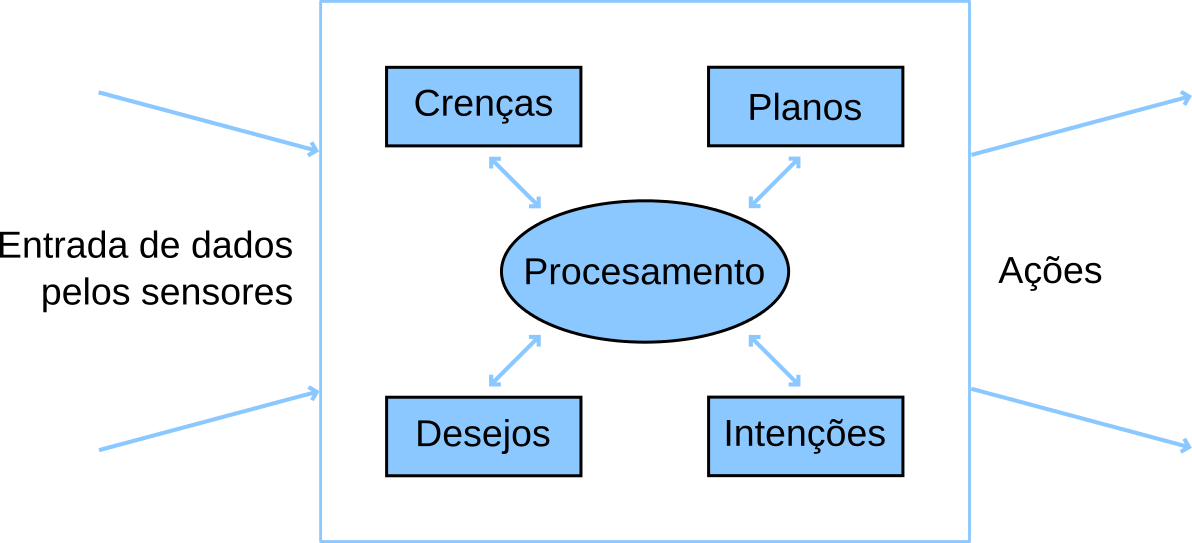
\includegraphics[width=3.3in]{BDI.png}
            \end{center}
            \caption{Arquitetura BDI, adaptada de \cite{weiss1999multiagent}}
            \label{fig:bdi}
        \end{figure}
        
        Os Sistemas Multiagentes (SMA) estudam o comportamento de um conjunto de agentes autônomos, eventualmente com características diferentes, evoluindo em um ambiente comum. Estes agentes podem interagir uns com os outros, com o objetivo de realizar suas tarefas de modo cooperativo, compartilhando informações, evitando conflitos e coordenando a execução de atividades \cite{alvares1997introduccao}.
        Para especificar agentes cognitivos é utilizada a linguagem \textit{AgenkSpeak}. Essa especificação é gerada através de um conjunto de crenças, planos, eventos que realizam a ativação e um conjunto de ações básicas que os agentes executam sobre determinado ambiente. Os programas escritos em AgenkSpeak  são interpretados de maneira semelhante á programas escritos em lógica prolog.      
        
    O objetivo desse artigo é analisar o tempo de execução de agentes, quando executados em computadores equipados com diferentes processadores da linha Intel Corporation. Para tal, este artigo está organizado da seguinte maneira: a Seção 2, é apresentada o estudo de caso e sua execução. Na Seção 3 são apresentados os resultados obtidos desse estudo e finalmente, a Seção 4 expõe a conclusão do trabalho.
      

    \section{Estudo de Caso}
    
    O cenário escolhido para execução do estudo de caso é conhecido como o vendedor de livros. Este cenário basicamente relaciona agentes com papéis de acordo com sua finalidade.  Agentes tem papéis de vendedores e compradores de livros. 
        
    Inicialmente, cada agente comprador recebe o título do livro para comprar como um argumento de linha de comando. Periodicamente, ele envia uma mensagem á todos os agentes vendedores conhecidos para fornecer uma oferta. Assim que uma oferta é recebida, o agente comprador aceita e emite uma ordem de compra. Se mais de um agente vendedor fornece uma oferta, o agente comprador aceita a melhor, no caso a proposta que apresentar um menor preço. Quando a compra é realizada, o agente comprador finaliza a execução.
        
    Vale ressaltar, que cada agente com papel de vendedor tem uma interface gráfica mínima, por meio do qual o usuário pode inserir novos títulos com preço associado no catálogo de livros para venda. Agentes vendedores esperam continuamente por pedidos de agentes compradores e quando solicitados a fornecerem uma oferta para um livro, os vendedores verificam se o livro solicitado está em seu catálogo. Neste caso, há uma resposta com preço do livro. Caso contrário, eles se recusam. Quando recebem uma ordem de compra corretamente, o agente vendedor remove o item do catálogo e finaliza a operação.
    
    O código dos agentes vendedores foi desenvolvido com a ferramenta Jason, do inglês (\textit{Java-based interpreter for an extended version of AgentSpeak}) consiste em um intérprete para uma versão estendida do \textit{AgentSpeak}. Ele implementa a semântica operacional da linguagem e fornece uma plataforma para o desenvolvimento de sistemas multi-agente, com muitas características de usuário personalizável. Jason está disponível \textit{Open Source} e é distribuído sob a licença GNU LGPL.
      
        Um SMA desenvolvido na ferramenta Jason, possui um ambiente onde os agentes estão situados e um conjunto de instâncias de agentes em \textit{AgentSpeak(L)}. O ambiente dos agentes, deve ser desenvolvido na linguagem Java.        
   
        A configuração do SMA é feita em arquivos com extensão .mas2j, basicamente é informado qual a arquitetura do SMA, "\textit{Centralized}" ou "Jade" (distribuída), qual o ambiente onde os agentes estão situados e os agentes em si. A programação dos agentes em AgentSpeak(L) é feita em arquivos com extensão .asl.
        
        O agente comprador é executado no JADE que é um framework em Java voltado para desenvolvimento de agentes. Basicamente é uma plataforma de código aberto para aplicações de agente com base em \textit{peer-to-peer}. Esse framework simplifica a implementação de sistemas multi-agente através de um \textit{middleware} que esteja em conformidade com as especificações do FIPA e através de um conjunto de ferramentas gráficas que suportam as fases de depuração e implantação. Um sistema baseado em JADE pode ser distribuído em máquinas (que não necessitam compartilhar o mesmo sistema operacional) e a configuração pode ser controlada através de uma interface gráfica (GUI).
        
        Por conseguinte, o JADE promove a importante integração com o Jason a fim de prover a interação e troca de mensagens entre os agentes executados. Na Figura \ref{fig:snifer} o \textit{Agent Sniffer} ilustra  através de um diagrama a troca de mensagens entre os agentes do cenário escolhido para execução.
        
		 \begin{figure}[ht]
            \begin{center}
                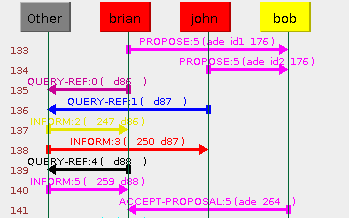
\includegraphics[width=3.3in]{sniffer}
            \end{center}
            \caption{Troca de mensagens entre agentes no JADE}
            \label{fig:snifer}
        \end{figure}
    
    
    \section{Ambiente de execução}
    
    Para o experimento foram utilizados dois computadores, sendo um \textit{notebook} e um \textit{desktop}. O \textit{notebook} possui um processador Intel Core i5-4210U \cite{inteli5} com 2 núcleos e 6 GB de RAM. O \textit{desktop} está equipado com um processador Intel Core i7 870 com 4 núcleos e 4 Gb de RAM. A Tabela \ref{tab:processadores} apresenta as especificações dos processadores. Todos os experimentos são executados no sistema operacional  Linux com a distribuição Linux Mint 17.3 e versão do \textit{kernel} 3.19.0.
        
        
        \begin{table}[ht]
            \caption{Especificações dos processadores utilizados \cite{inteli5} \cite{inteli7}}
            \begin{center}
                \begin{tabular}{l|l|l}
                    \hline
                    & Computador 1  & Computador 2 \\
                    \hline
                    Processador & Intel i5 4210U  & Intel i7 870 \\
                    \hline
                    Codinome Arch & Haswell  & Nehalem \\
                    \hline
                    Nº de Núcleos & 2 & 4\\
                    \hline
                    Nº de \textit{Threads} & 4 & 8\\
                    \hline
                    L1 Cache & 32K I, 32K D & 32K I, 32K D\\
                    \hline
                    L2 Cache & 256K & 256K\\
                    \hline
                    L3 Cache & 3072K & 8192K\\
                    \hline
                    Litografia & 22 nm & 45 nm\\
                    \hline
                    TDP & 15 W & 95 W\\
                    \hline
                    Frequência & Base 1.7GHz / Max 2.7GHz & Base 2,93GHz / Max 3,6GHz\\
                    \hline
                \end{tabular}
            \end{center}
            \label{tab:processadores}
        \end{table}        
    
    
    
        Os processadores utilizados no estudo de caso são componentes da empresa Intel Corporation e fazem parte de diferentes microarquiteturas. As microarquiteturas são evolutivas e apresentam algumas peculiaridades. Na Tabela \ref{tab:microarquitetura} são apresentadas as principais microarquiteturas Intel, o ano de lançamento e a litografia de cada uma.
        
        É possível observar que a cada evolução houve uma redução no tamanho da litografia, e esta redução permite um chaveamento mais rápido dos dispositivos, menor consumo de energia e maior fator de integração de dispositivos na mesma área do chip do processador. Permitindo que mais funcionalidades sejam acrescentadas \textit{on-chip}, como por exemplo mais memória cache interna.
                  
        Com apenas um núcleo e limitado apenas ao paralelismo a nível de instrução \textit{(ILP - Instruction Level Parallelism)} os processadores já não acompanhavam o crescimento desejado. O grande consumo de energia e a latência de memória eram obstáculos para um melhor desempenho em processadores com núcleo único utilizando o ILP. Com o surgimento de tecnologias de processadores multicore, houve um incremento no desempenho de diversos algoritmos explorando o paralelismo a nível de \textit{thread} \textit{(TLP - Thread Level Parallelism)}.
          
        \begin{figure}[ht]
        \centering
        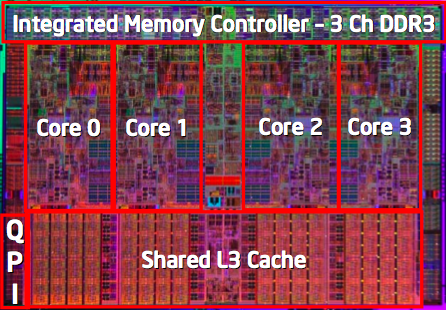
\includegraphics[width=2in]{nehalem-diagram}
        \caption{Microarquitetura Nehalem \cite{nehalemb}}
        \label{fig: figa}
        \end{figure}
        
        \begin{figure}[ht]
        \centering
        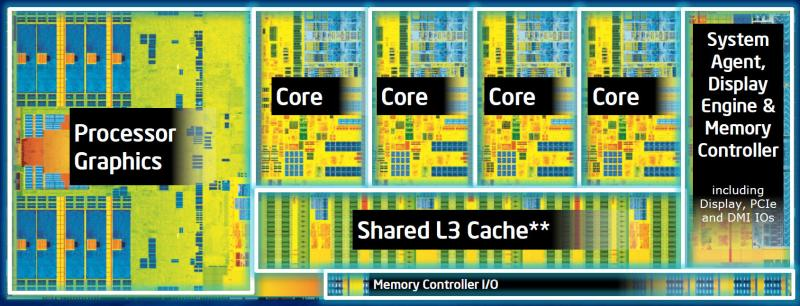
\includegraphics[width=3.5in]{haswell-diagram}
        \caption{Microarquitetura Haswell \cite{haswellb}}
        \label{fig: figb}
        \end{figure}
        
        
        Entre as microarquiteturas presentes nos computadores utilizados para execução do estudo de caso, foi analisada a evolução destes. Quando comparado ao Nehalem, o processador Haswell teve um grande impacto nas mudanças na hierarquia de memória, além do aumento da largura da banda de cache. Também, há um aumento nas operações de ponto flutuante por segundo (FLOPs - \textit{Floating-point Operations Per Second}) e novas unidades  de adição e multiplicação fundidas de ponto flutuante (FMA - \textit{Floating-Point Fused Multiply-Add})\cite{jain2013haswell}.
    

        \begin{figure}[ht]
            \centering
            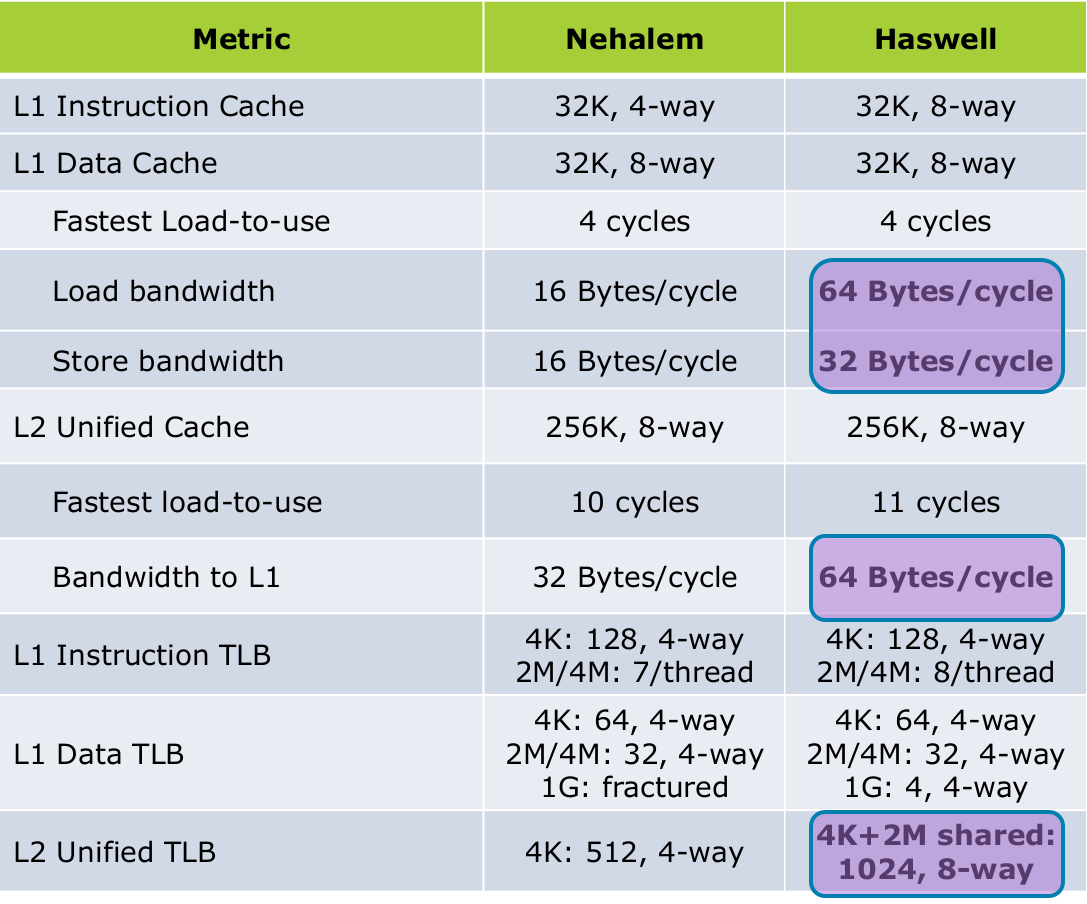
\includegraphics[width=3.5in]{nehalemvshaswell.png}
            \caption{Comparativo da hierarquia de memória Nehalem e Haswell, adaptada de \cite{hammarlund20134th}}
            \label{nhvshaswell}
        \end{figure}
        
        Na Figura \ref{hm} aprasentam-se as modificações que beneficiaram esse aumento de desempenho. Nas portas 0 e 1 foi acrescentado novas unidades de FMA. Na porta 6 uma unidade lógico aritmética (ALU - \textit{Arithmetic Logic Unit}) foi incrementada, este item é otimizado para trabalhar com inteiros. Enquanto as ALU das portas 0 e 1 preferencialmente trabalham com vetores. Ainda na porta 6 um novo \textit{Branch} reduz os possíveis conflitos na porta 0. Uma unidade geradora de endereços (AGU - \textit{Address Generation Unit}) é adicionada à porta 7. Esta AGU chamada de \textit{Store Address} libera as AGUs das portas 2 e 3 para trabalharem com carregamento de endereços, fazendo agora que este processador tenha capacidade de sustentar dois \textit{Loads} e um \textit{Store} por ciclo\cite{hammarlund20134th}.

        \begin{figure}[ht]
        \centering
        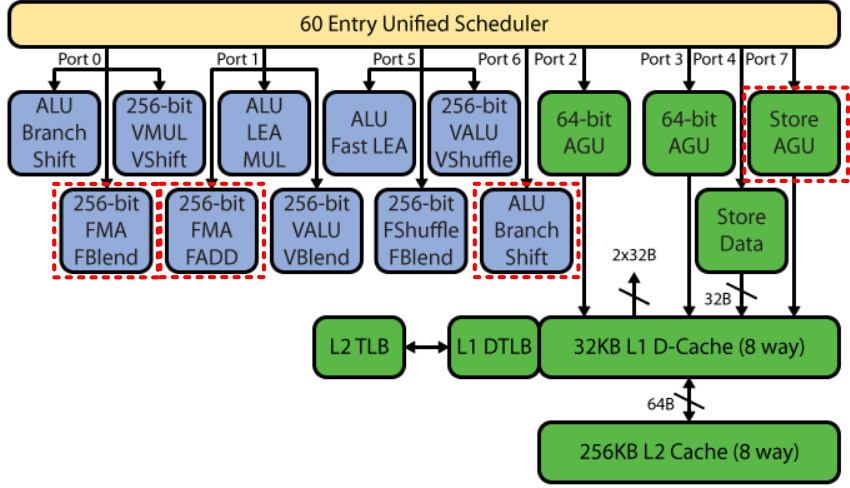
\includegraphics[width=3.5in]{haswell.png}
        \caption{Microarquitetura Haswell}
        \label{hm}
        \end{figure}
        
                \section{Resultados}
        
        O experimento baseou-se em executar o cenário proposto de forma descentralizada promovendo uma integração entre as ferramentas Jason e Jade. As execuções realizadas alteravam a quantidade de agentes inicializados em ambas as máquinas. Para simular o cenário dos agentes inseridos, iniciou-se com apenas um agente e encerrou-se com dez mil agentes no papel de vendedores como apresentado na Tabela \ref{tab:resultadostab}. Vale ressaltar que a média e o desvio padrão foram calculados após serem executadas dez rodadas de execução por quantidade de agentes. Observa-se que a variação após um número acima de dez mil agentes, há falta de \textit{hardware} para execução, pois a memória em uso girava em torno de 3200 mb. Quando apresentou um número superior, a memória Swap era utilizada. Este fato pode ocasionar problemas de desempenho decorrente da utilização dessa memória mais lenta.
        
\begin{table*}[ht]
\centering
\caption{Tempo de execução \textit{versus} nº de agentes}
\label{tab:resultadostab}
\begin{tabular}{|c|c|c|c|c|c|c|}
\hline
\multicolumn{1}{|l|}{Nº de Agentes} & \multicolumn{1}{l|}{Tempo Médio i7 (ms)} & \multicolumn{1}{l|}{Tempo Médio i5 (ms)} & \multicolumn{1}{l|}{Desvio Padrão i7} & \multicolumn{1}{l|}{Desvio Pradão i5} & \multicolumn{1}{l|}{Relação Desvio Padrão i7 e i5} & \multicolumn{1}{l|}{Relação Tempo Médio i7 e i5} \\ \hline
1                                   & 10045                                    & 10044                                    & 4,46                                  & 12,55                                 & 282\%                                              & 100,01\%                                         \\ \hline
2                                   & 10049                                    & 10052                                    & 14,4                                  & 13,83                                 & 96\%                                               & 99,97\%                                          \\ \hline
10                                  & 10064                                    & 10084                                    & 13,35                                 & 25,32                                 & 191\%                                              & 99,81\%                                          \\ \hline
50                                  & 10109                                    & 10216                                    & 15,73                                 & 61,12                                 & 391\%                                              & 98,95\%                                          \\ \hline
100                                 & 10165                                    & 10320                                    & 39,78                                 & 73,89                                 & 185\%                                              & 98,50\%                                          \\ \hline
200                                 & 10168                                    & 10334                                    & 33,69                                 & 95,1                                  & 282\%                                              & 98,40\%                                          \\ \hline
400                                 & 10188                                    & 10433                                    & 65,74                                 & 312,21                                & 474\%                                              & 97,65\%                                          \\ \hline
600                                 & 10189                                    & 10315                                    & 43,96                                 & 62,33                                 & 141\%                                              & 98,78\%                                          \\ \hline
1000                                & 10191                                    & 10315                                    & 32,88                                 & 49,36                                 & 150\%                                              & 98,80\%                                          \\ \hline
2000                                & 10195                                    & 10327                                    & 77,4                                  & 67,05                                 & 86\%                                               & 98,73\%                                          \\ \hline
5000                                & 10282                                    & 10561                                    & 214,38                                & 250,18                                & 116\%                                              & 97,36\%                                          \\ \hline
10000                               & 11209                                    & 13303                                    & 1034,18                               & 1077,25                               & 104\%                                              & 84,26\%                                          \\ \hline
\end{tabular}
\end{table*}        
        
        A coluna Relação Desvio Padrão i7 e i5 da Tabela \ref{tab:resultadostab} apresenta o quão estável estão os desvios padrões apresentados comparando os processadores Intel i7 e i5 nos testes com o mesmo número de agentes. No caso, quanto mais próximos de 100\% mais estável é a comparação. Isso serve para mostrar que, apesar do desvio padrão próximo 1000, quando existem 10000 agentes isso não é causado por falha de execução da pesquisa. O valor de 104\% indica que deve ser uma falha no próprio sistema em gerenciar tantos agentes, gerando assim uma variação muito alta no tempo das execuções.
        
        
        Na Figura \ref{grafico} apresenta-se o gráfico gerado com os dados obtidos. É possível observar que o desempenho da arquitetura i7 é superior ao da arquitetura i5, apresentando tempos inferiores em quase todos os casos estudados. Em ambientes com até 50 agentes, as duas arquiteturas apresentaram comportamento semelhante. Isso é relevante para destacar que, para situações com poucos agentes, a arquitetura i5 pode ser explorada com resultados adequados de desempenho. Entretanto, um número de 10.000 agentes executando há um aumento significativo no tempo de execução. O tempo de execução na arquitetura i7 é praticamente constante quando aumenta-se o número de agentes até o limite de 10000, onde observa-se um aumento no tempo de execução considerável. Pois, apesar da evolução na linha de processadores i5 e i7, a arquitetura i5 ainda é menos poderosa em desempenho quando executada no contexto com vários agentes.
        
        \begin{figure}[ht]
        \centering
        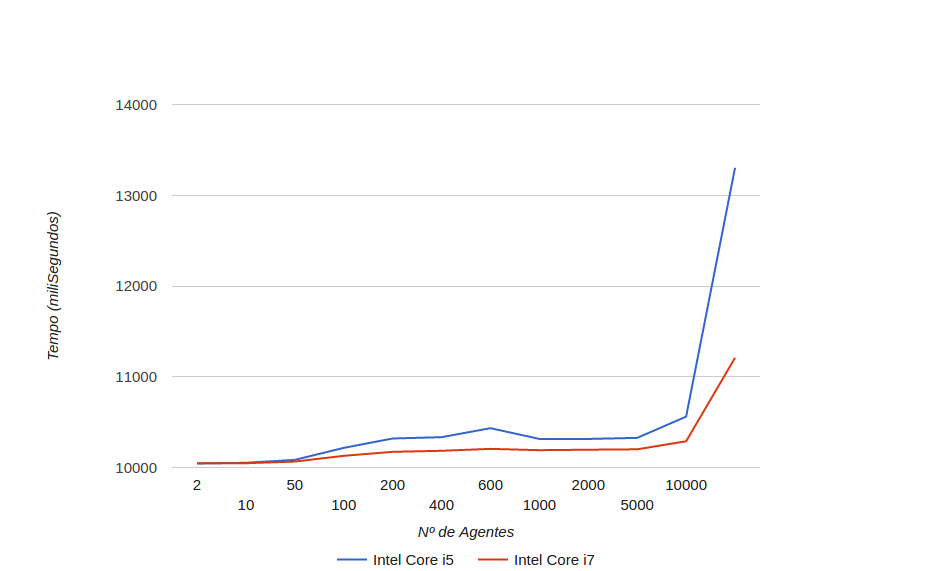
\includegraphics[width=3.5in]{grafico.png}
        \caption{Tempo de execução em relação ao nº de agentes}
        \label{grafico}
        \end{figure}
        
        
    \section{Conclusão}

        Agentes podem ser aplicados em diversos contextos e aplicações. Para esse trabalho, um problema simples baseado em agentes foi escolhido para o estudo de caso.  Analisando o tempo de execução nos vários cenários propostos, levando em consideração o número de agentes interagindo entre si, observa-se que a capacidade de processamento do maior número de cores e \textit{threads} do processador Intel Core i7 da microarquitetura Nehalem é muito superior ao Intel Core i5 apesar dos avanços da microarquitetura Haswell. \par
        Como trabalhos futuros, uma possibilidade é realizar esse estudo de caso utilizando mais agentes executando em \textit{Compute Unified Device Architecture} (CUDA). A CUDA é uma plataforma de computação paralela utilizada para tirar proveito das unidades de processamento gráficos (GPUs) de placas da NVIDIA, objetivando a resolução de problemas computacionais complexos que demorariam maior tempo para serem resolvidos em um processador convencional.        

% needed in second column of first page if using \IEEEpubid
%\IEEEpubidadjcol

% An example of a floating figure using the graphicx package.
% Note that \label must occur AFTER (or within) \caption.
% For figures, \caption should occur after the \includegraphics.
% Note that IEEEtran v1.7 and later has special internal code that
% is designed to preserve the operation of \label within \caption
% even when the captionsoff option is in effect. However, because
% of issues like this, it may be the safest practice to put all your
% \label just after \caption rather than within \caption{}.
%
% Reminder: the "draftcls" or "draftclsnofoot", not "draft", class
% option should be used if it is desired that the figures are to be
% displayed while in draft mode.
%
%\begin{figure}[!t]
%\centering
%\includegraphics[width=2.5in]{myfigure}
% where an .eps filename suffix will be assumed under latex, 
% and a .pdf suffix will be assumed for pdflatex; or what has been declared
% via \DeclareGraphicsExtensions.
%\caption{Simulation Results}
%\label{fig_sim}
%\end{figure}

% Note that IEEE typically puts floats only at the top, even when this
% results in a large percentage of a column being occupied by floats.


% An example of a double column floating figure using two subfigures.
% (The subfig.sty package must be loaded for this to work.)
% The subfigure \label commands are set within each subfloat command, the
% \label for the overall figure must come after \caption.
% \hfil must be used as a separator to get equal spacing.
% The subfigure.sty package works much the same way, except \subfigure is
% used instead of \subfloat.
%
%\begin{figure*}[!t]
%\centerline{\subfloat[Case I]\includegraphics[width=2.5in]{subfigcase1}%
%\label{fig_first_case}}
%\hfil
%\subfloat[Case II]{\includegraphics[width=2.5in]{subfigcase2}%
%\label{fig_second_case}}}
%\caption{Simulation results}
%\label{fig_sim}
%\end{figure*}
%
% Note that often IEEE papers with subfigures do not employ subfigure
% captions (using the optional argument to \subfloat), but instead will
% reference/describe all of them (a), (b), etc., within the main caption.


% An example of a floating table. Note that, for IEEE style tables, the 
% \caption command should come BEFORE the table. Table text will default to
% \footnotesize as IEEE normally uses this smaller font for tables.
% The \label must come after \caption as always.
%
%\begin{table}[!t]
%% increase table row spacing, adjust to taste
%\renewcommand{\arraystretch}{1.3}
% if using array.sty, it might be a good idea to tweak the value of
% \extrarowheight as needed to properly center the text within the cells
%\caption{An Example of a Table}
%\label{table_example}
%\centering
%% Some packages, such as MDW tools, offer better commands for making tables
%% than the plain LaTeX2e tabular which is used here.
%\begin{tabular}{|c||c|}
%\hline
%One & Two\\
%\hline
%Three & Four\\
%\hline
%\end{tabular}
%\end{table}


% Note that IEEE does not put floats in the very first column - or typically
% anywhere on the first page for that matter. Also, in-text middle ("here")
% positioning is not used. Most IEEE journals use top floats exclusively.
% Note that, LaTeX2e, unlike IEEE journals, places footnotes above bottom
% floats. This can be corrected via the \fnbelowfloat command of the
% stfloats package.

% if have a single appendix:
%\appendix[Proof of the Zonklar Equations]
% or
%\appendix  % for no appendix heading
% do not use \section anymore after \appendix, only \section*
% is possibly needed

% use appendices with more than one appendix
% then use \section to start each appendix
% you must declare a \section before using any
% \subsection or using \label (\appendices by itself
% starts a section numbered zero.)
%


% Can use something like this to put references on a page
% by themselves when using endfloat and the captionsoff option.
\ifCLASSOPTIONcaptionsoff
  \newpage
\fi



% trigger a \newpage just before the given reference
% number - used to balance the columns on the last page
% adjust value as needed - may need to be readjusted if
% the document is modified later
%\IEEEtriggeratref{8}
% The "triggered" command can be changed if desired:
%\IEEEtriggercmd{\enlargethispage{-5in}}

% references section

% can use a bibliography generated by BibTeX as a .bbl file
% BibTeX documentation can be easily obtained at:
% http://www.ctan.org/tex-archive/biblio/bibtex/contrib/doc/
% The IEEEtran BibTeX style support page is at:
% http://www.michaelshell.org/tex/ieeetran/bibtex/
%\bibliographystyle{IEEEtran}
% argument is your BibTeX string definitions and bibliography database(s)
%\bibliography{IEEEabrv,../bib/paper}
%
% <OR> manually copy in the resultant .bbl file
% set second argument of \begin to the number of references
% (used to reserve space for the reference number labels box)
\bibliographystyle{abbrv}
\bibliography{referencias}

% biography section
% 
% If you have an EPS/PDF photo (graphicx package needed) extra braces are
% needed around the contents of the optional argument to biography to prevent
% the LaTeX parser from getting confused when it sees the complicated
% \includegraphics command within an optional argument. (You could create
% your own custom macro containing the \includegraphics command to make things
% simpler here.)
%\begin{biography}[{\includegraphics[width=1in,height=1.25in,clip,keepaspectratio]{mshell}}]{Michael Shell}
% or if you just want to reserve a space for a photo:

%\begin{IEEEbiography}[{\includegraphics[width=1in,height=1.25in,clip,keepaspectratio]{picture}}]{John Doe}
%\blindtext
%\end{IEEEbiography}

% You can push biographies down or up by placing
% a \vfill before or after them. The appropriate
% use of \vfill depends on what kind of text is
% on the last page and whether or not the columns
% are being equalized.

%\vfill

% Can be used to pull up biographies so that the bottom of the last one
% is flush with the other column.
%\enlargethispage{-5in}




% that's all folks
\end{document}